\let\negmedspace\undefined
\let\negthickspace\undefined
\documentclass[journal]{IEEEtran}
\usepackage[a5paper, margin=10mm, onecolumn]{geometry}
%\usepackage{lmodern} % Ensure lmodern is loaded for pdflatex
\usepackage{tfrupee} % Include tfrupee package

\setlength{\headheight}{1cm} % Set the height of the header box
\setlength{\headsep}{0mm}     % Set the distance between the header box and the top of the text

\usepackage{gvv-book}
%\usepackage{gvv}
\usepackage{cite}
\usepackage{amsmath,amssymb,amsfonts,amsthm}
\usepackage{algorithmic}
\usepackage{graphicx}
\usepackage{textcomp}
\usepackage{xcolor}
\usepackage{txfonts}
\usepackage{listings}
\usepackage{enumitem}
\usepackage{mathtools}
\usepackage{gensymb}
\usepackage{comment}
\usepackage[breaklinks=true]{hyperref}
\usepackage{tkz-euclide} 
\usepackage{listings}
\usepackage{gvv}                                        
\def\inputGnumericTable{}                                 
\usepackage[latin1]{inputenc}                                
\usepackage{color}                                            
\usepackage{array}                                            
\usepackage{longtable}                                       
\usepackage{calc}                                             
\usepackage{multirow}                                         
\usepackage{hhline}                                           
\usepackage{ifthen}                                           
\usepackage{lscape}
\begin{document}

\bibliographystyle{IEEEtran}

\title{4.13.24}
\author{EE25BTECH11019 - Darji Vivek M.}
{\let\newpage\relax\maketitle}

\renewcommand{\thefigure}{\theenumi}
\renewcommand{\thetable}{\theenumi}
\setlength{\intextsep}{10pt}
\numberwithin{figure}{enumi}
\renewcommand{\thetable}{\theenumi}

\textbf{Question}:\\
The number of points, having both co-ordinates as integers, that lie in the interior of the triangle with vertices $(0,0)$, $(0,41)$ and $(41,0)$ is:

\begin{multicols}{4}
\begin{enumerate}
    \item 820
    \item 780
    \item 901
    \item 861
\end{enumerate}
\end{multicols}

\solution

\begin{align}
\vec{A} &= \myvec{0\\0}, &
\vec{B} &= \myvec{0\\41}, &
\vec{C} &= \myvec{41\\0}
\end{align}

\textbf{Step 1: Area using determinant.}
\begin{align}
A &= \frac{1}{2}\left|\mydet{0 & 41\\41 & 0}\right|\\
A &= \frac{1}{2}\left|0 - (41)(41)\right| \\
A &= \frac{1681}{2}
\end{align}

\textbf{Step 2: Boundary lattice points.}
For a line joining integer points $(x_1,y_1)$ and $(x_2,y_2)$,  
the number of lattice points on it is given by
\begin{align}
N &= \gcd(|x_2 - x_1|, |y_2 - y_1|) + 1
\end{align}

For each side:
\begin{align}
B_1 &= \gcd(|0 - 0|, |41 - 0|) + 1 = 41 + 1 = 42 \\
B_2 &= \gcd(|41 - 0|, |0 - 0|) + 1 = 41 + 1 = 42 \\
B_3 &= \gcd(|41 - 0|, |0 - 41|) + 1 = 41 + 1 = 42
\end{align}

Since each vertex is counted twice,
\begin{align}
B &= 42 + 42 + 42 - 3 = 123
\end{align}

\textbf{Step 3: Apply Pick's theorem.}
\begin{align}
A &= I + \frac{B}{2} - 1
\end{align}

Rearranging for $I$,
\begin{align}
I &= A - \frac{B}{2} + 1
\end{align}

Substitute $A = \frac{1681}{2}$ and $B = 123$:
\begin{align}
I &= \frac{1681}{2} - \frac{123}{2} + 1 \\
I &= \frac{1558}{2} + 1 \\
I &= 780
\end{align}

The number of integer lattice points lying strictly inside the triangle is
\boxed{780}


\begin{figure}[H]
\centering
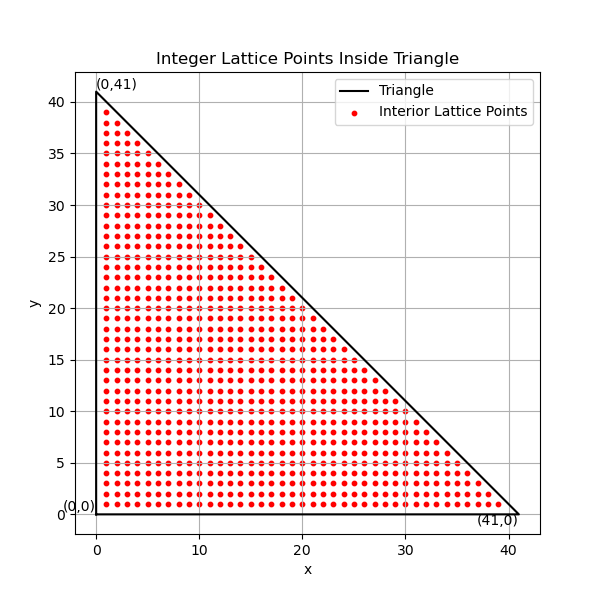
\includegraphics[width=0.75\columnwidth]{figs/9.png}
\caption{\centering plot}
\label{figs:traingle points}
\end{figure}

\end{document}
